\section{Evaluation Lösungsprinzipien}

Aus der vorhergehenden Technologierecherche wird pro Studiengang ein Morphologischer Kasten erstellt. Dieser wird befüllt mit den Teilfunktionen und den recherchierten Technologien. Damit werden die Lösungsprinzipien evaluiert und verschiedene Varianten werden gefunden. Ein Überblick ueber alle Morphologischen Kasten befindet sich im Anhang \ref{Morphologischer Kasten}.

\subsection{Maschinentechnik Morphologischer Kasten}

PLACEHOLDER

\subsection{Elektrotechnik Morphologischer Kasten}

PLACEHOLDER

\subsection{Informatik Morphologischer Kasten}

Aus der Technologierecherche wurde folgender Morphologischer Kasten mit drei Varianten für die Informatik Teilfunktionen erstellt.

\begin{figure}[H]
\centering
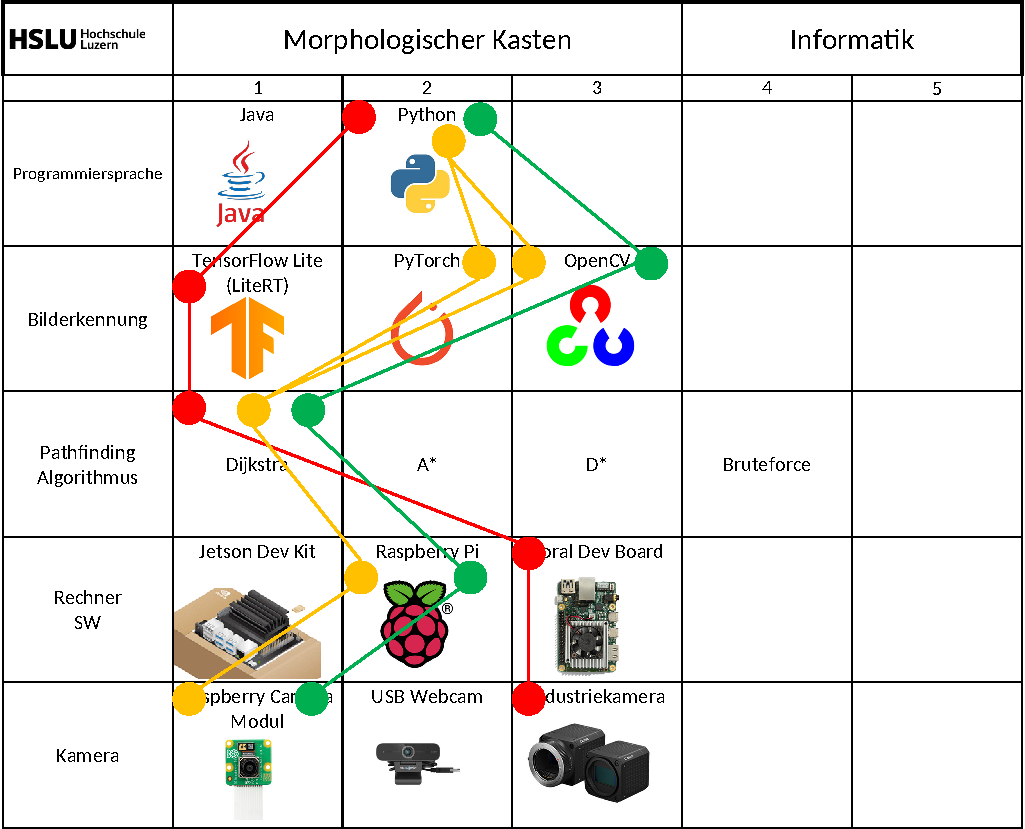
\includegraphics[width=\textwidth]{assets/MK_Informatik.pdf}
\caption{Morphologischer Kasten: Informatik}
\label{fig:mk-informatik}
\end{figure}

Es gibt nun drei Lösungskombinationen, die in einem nächsten Schritt evaluiert werden.

\begin{enumerate}
     \item Python verwendet eine Mischung aus PyTorch und OpenCV, um AI und reine Bilderkennung zu verwenden. Dijkstra berechnet den Weg. Das Ganze rechnet auf einem Raspberry Pi mit einer Raspberry Camera angeschlossen.
    \item Python verwendet LiteRT, um mit AI die Umgebung zu erkennen und Dijkstra, um den Weg zu berechnen. Das Ganze rechnet auf einem Coral Dev Board und fotografiert den Graphen mit einer Industriekamera.
    \item  Python verwenden nur OpenCV zur Bilderkennung und berechnet mit Dijkstra den Weg, es rechnet auf einem Raspberry Pi mit einer Raspberry Camera.
\end{enumerate}

Bei den drei Varianten fällt auf, dass alle Python und den Wegfindealgorithmus Dijkstra verwenden würden. Python wurde immer gewählt, da Bilderkennung und Machine Learning sehr gut mit Python harmonisieren. Viele Libraries, inklusive dieser, die hier ersichtlich sind, sind kompatibel mit Python. Dijkstra wurde immer gewählt, weil dieser Algorithmus simpel und robust ist und die Geschwindigkeit vernachlässigbar ist. Da es im Graphen nur 8 Knoten gib, wird die Berechnung bei jedem Algorithmus schnell sein.

\subsection{Simulator Morphologischer Kasten}


Aus der Technologierecherche wurde folgender Morphologischer Kasten für die Teilfunktonen des Simulators erstellt. Es gibt drei Varianten, die in Frage kommen.

\begin{figure}[H]
\centering
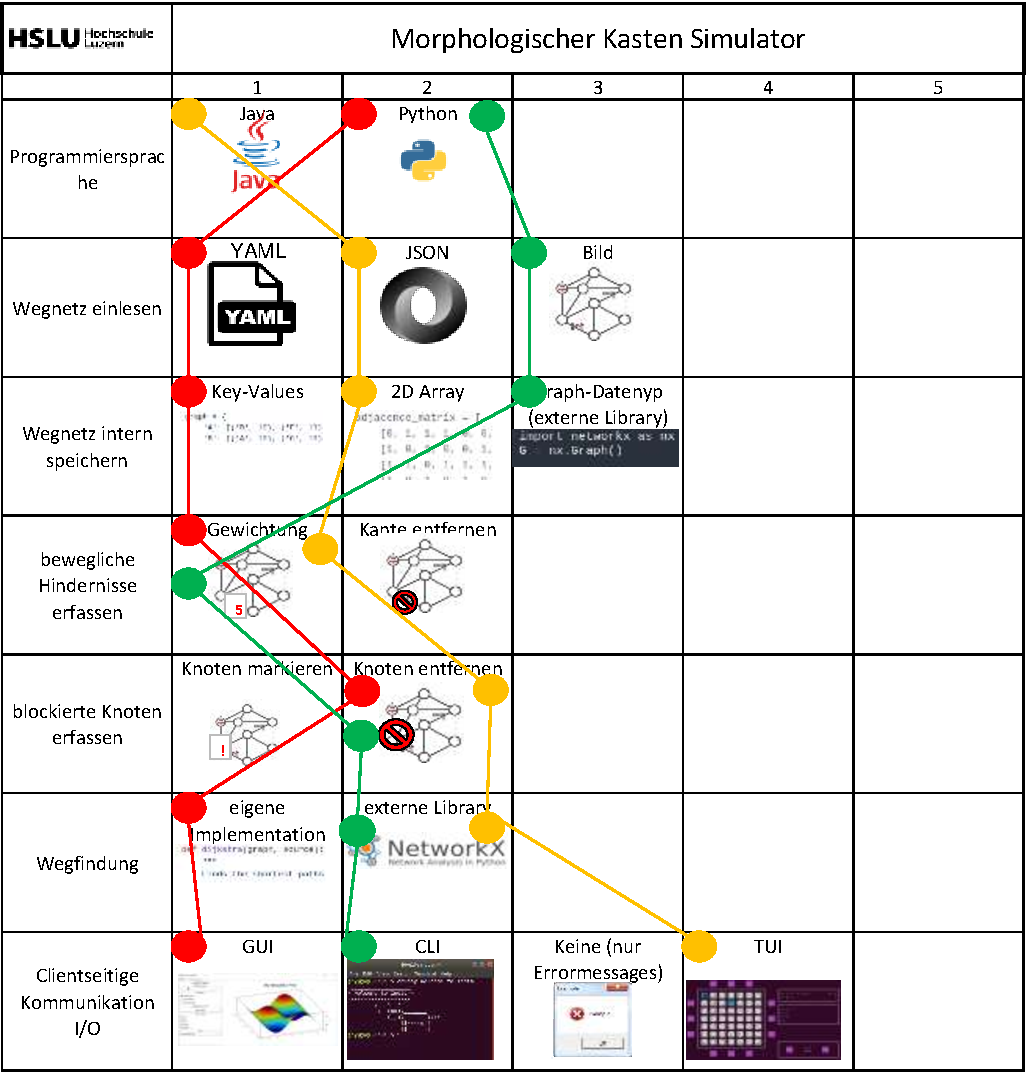
\includegraphics[width=\textwidth]{assets/MK_Simulator.pdf}
\caption{Morphologischer Kasten: Simulator}
\label{fig:mk-simulator}
\end{figure}

Die folgenden drei Lösungskombinationen, werden im nächsten Schritt evaluiert.

\begin{enumerate}
    \item Ein Java Simulator liest ein JSON File und speichert es in einem 2D Array. Bei einem beweglichen Hindernis wird die Gewichtung der Kante erhöht, bei einem Pylonen wird der Knoten entfernt. Dijkstra wird mit einer externen Library implementiert. Die Auswahl des Zielknotens erfolgt zufällig und die Aktivitäten des Roboters werden in einem TUI dargestellt.
    \item Ein Python Simulator liest ein YAML File und speichert es in einem Dictionary. Bei einem beweglichen Hindernis wird die Gewichtung der Kante erhöht, bei einem Pylonen wird der Knoten entfernt. Dijkstra wird selber implementiert, das Ziel kann vom Menschen und zufällig ausgewählt werden und die Aktivitäten des Roboters sind in einem GUI ersichtlich.
    \item Ein Python Simulator liest ein Bild ein und speichert es in einem Graph Datentyp. Bei einem beweglichen Hindernis wird die Gewichtung der Kante erhöht, bei einem Pylonen wird der Knoten entfernt. Eine externe Library implementiert Dijkstra, das Ziel wird manuell ausgwählt und die Aktivitäten des Roboters werden in einem CLI dargestellt.
\end{enumerate}

In jeder Lösungsvariante wird die Kante nicht entfernt, sondern neu gewichtet bei einem beweglichen Hindernis. Dies liegt daran, dass es zu risikobehaftet wäre im Falle, dass es sonst keinen Weg geben würde. Die spräche gegen das Prinzip der Robustheit.

Ebenfalls wird ein Knoten immer entfernt, falls ein Pylon darauf steht und nicht markiert. Es würde keinen Vorteil bringen, den Knoten weiterhin zu speichern.


\newpage
\section{Auswahl Lösungskombinationen}

Zur Auswahl der passendsten Lösungskombination wird pro Teilbereich eine Nutzwertanalyse durchgeführt. Die Kriterien und deren Gewichtung sind individuell pro Teilbereich, damit sie ideal passen. Die Variante mit der höchsten Punktezahl ist die Variante, die am besten passt.

\subsection{Maschinentechnik Nutzwertanalyse}

PLACEHOLDER

\subsection{Elektrotechnik Nutzwertanalyse}

PLACEHOLDER

\subsection{Informatik Nutzwertanalyse}

Die drei ermittelten Varianten aus dem vorherigen Kapitel werden analysiert und bewertet mithilfe einer Nutzwertanalyse.

TODO BILD

Aus der Nutzwertanalyse kann abgelesen werden, dass die Variante B mit Python, PyTorch und OpenCV am besten passt. Die detaillierte Variante ist eingezeichnet in diesem Morphologischen Kasten.

TODO BILD VARIANTE IN KASTEN

\subsection{Simulator Nutzwertanalyse}

Die drei Varianten, wie der Simulator umgesetzt werden könnte, werden bewertet in folgender Nutzwertanalyse. Die Kriterien und deren Gewichtung sind dieselben, wie bei der Nutzwertanalyse für die Informatik im Roboter. Das Ziel des Simulators ist es, diesen möglichst realistisch und wiederverwendbar für \acrshort{pren2} umzusetzen.

TODO BILD

Die Nutzwertanalyse zeigt, dass die Variante B: Python mit YAML und einem GUI am besten abschneidet. Diese Variante besteht aus folgenden Teilen.


\begin{figure}[H]
\centering
\includegraphics[width=\textwidth]{assets/Morphologisches-Tableau.pdf}
\caption{Loesungskombination: Simulator}
\label{fig:mk-simulator-final}
\end{figure}
